\documentclass[12pt]{article}
\usepackage[utf8]{inputenc}
\usepackage{amsmath,amssymb,hyperref,array,xcolor,multicol,verbatim,mathpazo,algorithm,algpseudocode,enumerate,tikz}
\usepackage[normalem]{ulem}
\usepackage{graphicx}

\newenvironment{problem}[2][Problem]{\begin{trivlist}
\item[\hskip \labelsep {\bfseries #1}\hskip \labelsep {\bfseries #2.}]}{\end{trivlist}}

\begin{document}

%%%% In most cases you won't need to edit anything above this line %%%%

\title{\vspace{-4cm}CS 270 Homework 8}
\author{Neel Gupta} 
\maketitle

\begin{problem}{1}
    The following graph G has labeled nodes and edges between it. Each edge is labeled with its capacity.
    \begin{enumerate}[(a)]
        \item Draw the final residual graph $G_f$ using the Ford-Fulkerson algorithm corresponding to the max flow.
        \item What is the max-flow value?
        \item What is the min-cut?
    \end{enumerate}
    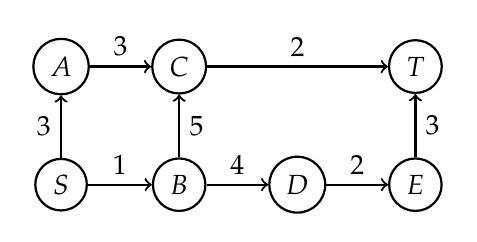
\begin{tikzpicture}[node distance={15mm}, thick, main/.style = {draw, circle}] 
        \node[main] (S) {$S$}; 
        \node[main] (A) [above of=S] {$A$};
        \node[main] (B) [right of=S] {$B$}; 
        \node[main] (C) [right of=A] {$C$};
        \node[main] (D) [right of=B] {$D$};
        \node[main] (E) [right of=D] {$E$};
        \node[main] (T) [above of=E] {$T$};
        \draw[->] (S)--(B) node [midway,above] {1};
        \draw[->] (S)--(A) node [midway,left] {3};
        \draw[->] (A)--(C) node [midway,above] {3};
        \draw[->] (B)--(C) node [midway,right] {5};
        \draw[->] (B)--(D) node [midway,above] {4};
        \draw[->] (D)--(E) node [midway,above] {2};
        \draw[->] (C)--(T) node [midway,above] {2};
        \draw[->] (E)--(T) node [midway,right] {3};
    \end{tikzpicture} 
\end{problem}

\textit{Answer:}

(a) There are 3 unique paths: $S \rightarrow A \rightarrow C \rightarrow T$, $S \rightarrow B \rightarrow D \rightarrow E \rightarrow T$, and $S \rightarrow A \rightarrow C \rightarrow B \rightarrow D\rightarrow E \rightarrow T$. Leaving below $G_f$.
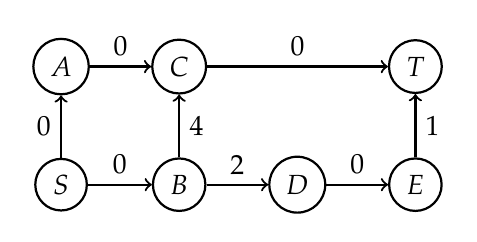
\begin{tikzpicture}[node distance={15mm}, thick, main/.style = {draw, circle}] 
    \node[main] (S) {$S$}; 
    \node[main] (A) [above of=S] {$A$};
    \node[main] (B) [right of=S] {$B$}; 
    \node[main] (C) [right of=A] {$C$};
    \node[main] (D) [right of=B] {$D$};
    \node[main] (E) [right of=D] {$E$};
    \node[main] (T) [above of=E] {$T$};
    \draw[->] (S)--(B) node [midway,above] {0};
    \draw[->] (S)--(A) node [midway,left] {0};
    \draw[->] (A)--(C) node [midway,above] {0};
    \draw[->] (B)--(C) node [midway,right] {4};
    \draw[->] (B)--(D) node [midway,above] {2};
    \draw[->] (D)--(E) node [midway,above] {0};
    \draw[->] (C)--(T) node [midway,above] {0};
    \draw[->] (E)--(T) node [midway,right] {1};
\end{tikzpicture} 

(b) The max-flow is 4.

(c) The min-cut crosses the edges $C\rightarrow T$ and $D \rightarrow E$, as this cut prevents all flow while minimizing the number of edges and weights lost.

\begin{problem}{2}
    Determine if the following statements are true or false. For each statement briefly explain your reasoning.
    \begin{enumerate}[(a)]
    \item In a flow network, the value of flow from S to T can be higher than the maximum number of edge disjoint paths from S to T. (Edge disjoint paths are paths that do not share any edge.)
        \item For a flow network, there always exists a maximum flow that doesn't include a cycle containing positive flow.
        \item If you have non-integer edge capacities, then you cannot have an integer max flow.
        \item Suppose the maximum s-t flow of a graph has value $f$. Now we increase the capacity of every edge by 1. Then the maximum s-t flow in this graph will have a value of at most $f+1$.
        \item If all edges are multiplied by a positive number $k$, then the min-cut remains unchanged.
    \end{enumerate}
\end{problem}

\textit{Answer:}

(a) \textbf{True.} The flow value can be higher than the number of edge-disjoint paths because the flow can be split between multiple paths, allowing for a larger total flow value.

(b) \textbf{True.} The max flow can always be achieved without cycles containing positive flow since any flow in a cycle can be rerouted to eliminate the cycle without affecting the overall flow's value.

(c) \textbf{False.} Even with non-integer edge capacities, it is still possible to have an integer max flow since non-integers can sum to integers. Consider a simple graph with two edges from S to T with capacities 0.5 and 1.5. The max flow is 2, which is an integer. 

(d) \textbf{False.} If we increase the capacity of every edge by 1, the maximum s-t flow can increase by more than 1. Consider a graph with a max flow split between 2 different paths. Then the max flow will increase by 2 since the minimum capacity on each path has now increased by 1 which is greater than 1.

(e) \textbf{True.} Scaling all edge capacities by the same positive factor $k$ does not change the structure of the graph. Therefore, the min-cut stays the same. However, the capacity of the min-cut will be scaled by $k$, even though its location does not change.

\begin{problem}{3}
    You are given a flow network with unit-capacity edges. It consists of a directed graph $G=(V,E)$ with a source s and sink t, and $c_e=1$ for every edge $e$. You are also given a positive integer parameter $k$. The goal is to delete $k$ edges so as to reduce the maximum s-t flow in $G$ by as much as possible. In other words, you should find a subset of edges $F \subseteq E$ such that $|F|=k$ and the maximum s-t flow in the graph $G=(V,E\setminus F)$ is as small as possible. Give a polynomial-time algorithm to solve this problem and briefly explain its correctness.

    Follow up: If the edges have more than unit capacity, will your algorithm produce the smallest possible max-flow value?
\end{problem}

\textit{Answer: }

\begin{enumerate}
    \item Compute the maximum flow of $G$ say $g$ using the Ford-Fulkerson algorithm because we will need to determine the initial max-flow value and min-cut.
    \item Find the min-cut of the s-t flow using min-cut max-flow theorem, which states that the max-flow value is equal to the capacity of the min-cut. The min-cut represents the bottleneck in the s-t flow.
    \item If $g\leq k$, remove all edges in the min-cut, disconnecting s and t, thus reducing the max-flow to 0. This is optimal since use we are allowed to remove at most $k$ edges, so removing all edges in the min-cut will ensure no flow occurs.
    \item If $g>k$, remove $k$ edges from the min-cut, creating a cut with a capacity of $g-k$. Since all edge capacities are 1, this will reduce the network flow by $k$, which is the maximum possible reduction given the constraints.
    \item The new graph has a max-flow of $g'=\text{max}(0,g-k)$. This is the smallest possible max-flow after removing $k$ edges.
\end{enumerate}

This algorithm runs in polynomial time because the Ford-Fulkerson algorithm has polynomial complexity, and finding the min-cut and removing $k$ edges each take polynomial time.

Follow up: If the edges have more than unit capacity, the algorithm may not produce the smallest possible max-flow value because the edge capacities will not directly correspond to the number of edge-disjoint paths. In this case, we need to consider edge capacities and possibly update the algorithm to remove edges with higher capacities first to minimize the max-flow value.

\begin{problem}{4}
    A tourist group needs to convert their USD into various international currencies. There are $n$ tourists $t_1, t_2, ..., t_n$ and $m$ currencies $c_1, c_2, ..., c_m$. Each tourist $t_i$ has $F_i$ dollars to convert. For each currency $c_j$, the bank can convert at most $B_j$ dollars to $c_j$. Tourist $t_i$ is willing to trade as much as $S_{ij}$ of his dollars for currency $c_j$. (For example, a tourist with 1000 dollars might be willing to convert up to 200 of his USD for Indian Rupees, up to 500 of his USD for Japanese Yen, and up to 300 USD for Euros.) Assume that all tourists give their requests to the bank at the same time.
    \begin{enumerate}[(a)]
        \item Design an algorithm that the bank can use to satisfy all the requests (if it is possible). To do this, construct and draw a network flow graph, with appropriate source and sink nodes, and edge capacities.
        \item Prove your algorithm is correct by making a claim and proving it in both directions.
    \end{enumerate}
\end{problem}

\textit{Answer:}

(a) We express this problem as a network flow problem. The idea for the problem is that we create a flow graph, where the fluid is dollars and the allocation of flow shows how this is transferred into different currencies.

The graph has nodes $x_1, x_2, ..., x_n$ for the tourists and $y_1, y_2, ..., y_m$ for the currencies. The source $s$ is connected to $x_1, x_2, ..., x_n$ and the nodes $y_1, y_2, ..., y_m$ are connected to the sink $t$. There are edges from the nodes  $x_1, x_2, ..., x_n$ to the nodes $y_1, y_2, ..., y_m$.

An edge $(s, x_i)$ has capacity $F_i$, the edges $(x_i, y_j)$ have capacity $S_{ij}$, and the edges $(y_j, t)$ have capacities $B_j$. A flow corresponds to converting dollars into different currencies. The capacity constraints ensure that the tourists and banks don't exceed the amounts of currency, and that the traders get appropriate currencies. If the maximum flow is equal to the sum of all the dollars tourists want to convert ($\sum_{i=1}^{n} F_i$), then it is possible to satisfy all the requests. Otherwise, it is not possible.

(b) Proof of correctness:

If the max-flow is equal to the sum of all dollars tourists want to convert, then it is possible to satisfy all the requests. 

The max-flow in the network represents the total amount of money that can be converted based on tourists' requests and the bank's capacity. If the maximum flow is equal to the sum of all the dollars tourists want to convert, it means that all requests can be satisfied without exceeding the bank's currency conversion capacities.

If it is possible to satisfy all the requests, then the max-flow in the constructed flow network is equal to the sum of all the dollars tourists want to convert.

In the constructed flow network, the edge capacities represent the tourists' requests and the bank's currency conversion capacities. If all requests can be satisfied, the flow from the source to the sink must be equal to the sum of all the dollars the tourists want to convert, which present the maximum flow in the network.

Since both directions are proven, the algorithm is correct. $\square$

\begin{problem}{5}
You have successfully computed a maximum $s-t$ flow $f$ for a network $G=(V,E)$ with integer edge capacities. Your boss now gives you another network $G'$ that is identical to $G$ except that the capacity of exactly one edge has decreased by one. You are also explicitly given the edge whose capacity was changed. Describe how you can compute a maximum flow for $G'$ in $O(|V|+|E|)$ time.
\end{problem}

\textit{Answer:}

\begin{enumerate}
\item Let $G=(V,E)$ be the original network, $G'=(V,E')$ be the modified network with one edge capacity decreased by 1, and $e=(u,v)$ be the edge whose capacity was changed.
\item Compute the max-flow $f$ for $G$ and obtain the residual graph $G_f$.
\item Update the residual graph $G_f$ by decreasing the capacity of the edge $e$ by 1. Let us denote this updated residual graph as $G_f'$.
\item Now, there might be a residual capacity of 1 in the reverse edge $(v, u)$ in $G_f'$.
\item If there's no augmenting path from $s$ to $t$ in $G_f'$, the current flow $f$ in $G_f'$ is a maximum flow for $G'$.
\item If there is an augmenting path from $s$ to $t$ in $G_f'$ that uses the reverse edge $(v, u)$, find the bottleneck capacity of the augmenting path, say $b$. Since the reverse edge has a capacity of 1, we can be sure that $b \leq 1$. Augment the flow in $G_f'$ along the found augmenting path with bottleneck capacity $b$ and obtain the new residual graph $G_f''$.
\end{enumerate}

Since the algorithm involves modifying the residual graph, finding an augmenting path, and augmenting the flow, which all take $O(|V|+|E|)$ or $O(|V|)$ time, the overall time complexity of this algorithm is $O(|V|+|E|)$.
\end{document}